\section{Results and Analysis}
\label{sec:results}

This section includes the main results for inconsistency detection and faithfulness rating, together with an ablation study, an analysis of error types, and comparisons of different model sizes of our FFLM. We also discussed our metric and the prompting approach with or without instruction tuning under the same model size.

\subsection{Performance on Inconsistency Detection}
\label{sec:results-id}


\begin{table*}[t]
	\scriptsize
	\centering
	\begin{tabular}{l|rrrrrr}
		\toprule[1pt]
		%\multirow{2}{*}{Model} & CoGenSum & SummEval & FRANK & PolyTope & FactCC & Xsumfaith \\
		% & \\ % three correlations 
		Metric & CoGenSum & SummEval & FRANK & Polytope & FactCC & XSumFaith \\
		\hline
		NER Overlap & 53.0 & 56.8 & 60.9 & 52.0 & 55.0 & 63.3 \\
		MNLI-doc &  57.6 & 66.6 & 63.6 & 61.0 &61.3 & 57.5 \\
		FactCC$_{\rm CLS}$ & 63.1 & 60.1 & 59.4 & 61.0 & 75.9 & 57.6 \\
		DAE & 63.4 & 70.3 & 61.7 & {62.8} & 75.9 & 50.8 \\
		FEQA & 61.0 & 53.8 & 69.9 & 57.8 & 53.6 & 56.0 \\
		QuestEval & 62.6 & 72.5 & 82.1  & \textbf{70.3} & 66.6 & 62.1 \\
		SummaC$_{\rm ZS}$ &70.4 & 78.7& 79.0& 62.0&83.8 &58.4  \\
		SummaC$_{\rm Conv}$ & 64.7&81.7 &81.6 &62.7 &\textbf{89.5} &\textbf{66.4} \\
		BARTScore & 62.5& 66.7&80.2 & 57.3& 68.4 & 56.9\\
		CoP$_{\rm BART}$ &  65.3 & 63.9 & 77.7 & 60.0 & 69.0 & 61.5\\
		HaRiM$_{\rm BART}$ & 58.9 &76.6 &81.8 &55.8 &67.3 &56.2\\
		ChatGPT &63.3 & 76.5& 80.9& 56.9& 74.7& {64.7}\\
		%ChatGPT$_{ZS-COT}$ &74.3 &83.3 &82.6 &61.4 &79.5 & 63.1 \\
		\hline
		CoP$_{\rm LLaMa}$ & 65.4 & 83.6 & 83.1 & 55.4 & 78.6 & 54.1 \\
		HaRiM$_{\rm LLaMa}$ & 57.1 & 80.0 & 83.4 & 58.8 & 69.8 & 53.4 \\
		FFLM & \underline{\textbf{71.8}} & \underline{\textbf{84.4}} & \underline{\textbf{83.9}} & \underline{61.5} &77.3  &\underline{58.9} \\
		\bottomrule[1pt]
	\end{tabular}
	\caption{Balanced accuracy(\%) on the SUMMAC benchmark. The best result for each dataset is in bold. Scores of FFLM better than other metrics based on the foundation model are underlined.}
	\label{tab:classification}
\end{table*}




\begin{table*}[h]
	\scriptsize
	\centering
	\begin{tabular}{l|ccc|ccc|ccc|ccc|ccc}
		\toprule[1pt]
		  & \multicolumn{3}{c}{FRANKCNN} & \multicolumn{3}{c}{QAGSCNN} &  \multicolumn{3}{c}{SummEval}  & \multicolumn{3}{c}{FRANKXSUM}  & \multicolumn{3}{c}{QAGSXSUM} \\
		 Metric & $\gamma$ &$\rho$ & $\tau$ & $\gamma$ &$\rho$ & $\tau$ & $\gamma$ &$\rho$ & $\tau$ & $\gamma$ &$\rho$ & $\tau$ & $\gamma$ &$\rho$ & $\tau$ \\
		\hline
		Rouge-2&  33.1 & 32.7 & 24.9 & 47.5 & 42.7 & 31.5 & 24.7 & 25.2 & 19.5 & 1.2 & 3.3 & 2.7 & 10.7 & 9.1 & 6.9 \\
		Meteor& 23.0 & 22.9 & 17.4 & 27.7 & 32.4 & 23.4 & 14.3 & 12.2 & 11.2 & -0.5 & 0.5 & 0.4 & -1.5 & -7.1 & -5.2 \\
		BLEU & 9.3 & 20.2 & 15.3 & 18.0 & 33.7 & 24.5 & 11.7 & 7.3 & 9.1 & -4.2 & -4.6 & -3.8 & 4.7 & -18.6 & -13.9 \\
		BERTScore &  51.4 &46.4& 35.8 & 55.6& 49.3& 36.5 & 29.2& 29.5& 23.0 &15.7 & 13.7 & 11.1 & -4.8 &-5.4 & -4.0\\
		%51.3 & 46.5 & 30.1 & 54.8 & 49.3 & 33.1 & 33.8 & 35.0 & 26.6 & 19.6 & 17.6 & 3.8 & -2.6 & -2.8 & -3.9 \\
		FactCC$_{\rm CLS}$ & 49.2 & 43.8 & 37.6 & -&- &- & 32.0 & 34.0 & - & 7.2 & 7.2 & 7.1 & -&- &- \\
		FEQA & -1.8 & -1.0 & -0.8 &- &- &- &- &- &- & 2.6 & 0.8 & 0.6 & -&- &- \\
		QAGS & 31.4 & 26.7 & 20.6 & 46.6 & 38.2 & 27.4 & 17.7 & 12.7 & - & -2.2 & -0.7 & -0.6 & 21.7 & 20.3 & 15.3 \\
		QuestEval &- &- &- & 49.2 & 44.5 & - & 37.0 & 33.9 & - &- & -& -& 7.0 & 9.6 & - \\
		DAE & 44.0 & 44.7 & 34.2 & -& -&- & 20.0 & 27.0 & - & 5.8 & 11.3 & 9.2 & -& -& -\\
		BARTScore & 56.1 & 53.0 & 41.3 & 67.3 & 61.3 & 47.0 & 24.9 & 26.2 & 19.7 & 17.4 & 16.8 & 13.7 & 8.0 & 9.7 & 7.2 \\
		CoP$_{\rm BART}$ & 56.1 & 51.0 & 39.4 & 73.0 & 65.3 & 53.2 & 23.6 & 22.6 & 18.0 & 22.8 & 20.8 & 17.0 & 26.6 & 25.3 & 20.7 \\
		HaRiM$_{\rm BART}$  & 61.0 & 53.9 & 42.1 & 67.4 & 58.2 & 47.1 & 42.7 & 37.6 & 29.8 & 14.8 & 13.9 & 11.4 & 15.8 & 16.0 & 13.1 \\ 
		ChatGPT & 50.0 & 46.0 & - & - & - & - & 49.0 & 35.0 & - & \textbf{34.0} & \textbf{27.0} & - & - & - & - \\ % ChatGPT as a Factual Inconsistency Evaluator for Abstractive Text Summarization
		\hline
		CoP$_{\rm LLaMa}$  & 59.7 & 54.5 & 42.6 & \textbf{74.3} & \textbf{67.6} & \textbf{54.8} & 55.1 & 46.4 & 37.0 & 24.6 & 23.1 & 18.8 & 19.0 & 18.1 & 14.7 \\
		HaRiM$_{\rm LLaMa}$ & 56.9 & 51.9 & 40.3 & 68.6 & 60.0 & 48.2 & 56.1 & 45.5 & 36.4 & 18.6 & 16.7 & 13.6 & 9.1 & 10.0 & 8.2\\
		FFLM & \underline{\textbf{62.2}} & \underline{\textbf{56.0}} & \underline{\textbf{43.7}} & 72.3 & 65.3 & 53.0 & \underline{\textbf{56.3}} & \underline{\textbf{46.9}} & \underline{\textbf{37.4}} & \underline{27.0} & \underline{25.3} & \underline{20.6} & \underline{\textbf{28.3}} & \underline{\textbf{27.1}} & \underline{\textbf{22.2}} \\
		\bottomrule[1pt]
	\end{tabular}
	\caption{Summary-level correlations(\%) on the faithfulness rating datasets.}
	\label{tab:correlation}
\end{table*}



The results on inconsistency detection are in Table~\ref{tab:classification}. 
Our proposed metric FFLM achieves state-of-the-art performance on 3 datasets including CoGenSum, SummEval, and FRANK, and outperforms ChatGPT on 5 out of 6 datasets from the SUMMAC benchmark except XSumFaith.

Both Polytope and FactCC are only labeled by a single annotator. As a result, 
their labels may not be as convincing as the other datasets. 
Although QuestEval, the best QA-based metric,  achieves the top-1 accuracy on Polytope, it performs mediocrely on the rest. The weakly-supervised baselines FactCC$_{\rm CLS}$ and SummaC$_{\rm Conv}$ are trained with synthetic data constructed with human expertise that may have certain similarities with the FactCC dataset. Therefore, FactCC$_{\rm CLS}$ shows strong performance on the FactCC dataset while relatively weak on the others including datasets in Table~\ref{tab:correlation}, the same as the findings in~\citet{laban2022summac}. Also, that's why SummaC$_{\rm Conv}$ shows around 12\% significant improvements over our FFLM. 

Concentrating on the metrics based on probability changes, zero-shot metrics CoP$_{\rm BART}$ and HaRiM$_{\rm BART}$ perform not badly compared with previous SOTA SummaC$_{\rm ZS}$, showing the potential of using probability changes for faithfulness evaluation. 
After introducing the foundation language model, their performances don't drop in most cases, indicating that fine-tuning with in-domain data is not necessary.
However, the leading performance between these two metrics is unstable among datasets. HaRiM$_{\rm LLaMa}$ outperforms CoP$_{\rm LLaMa}$ on FRANK and Polytope, while on the rest datasets, the opposite is true. FFLM, as a comprehensive metric, successfully achieves improvements over both of them on 5 out of 6 datasets.




\subsection{Performance on Faithfulness Rating}
\label{sec:results-fr}




Summary-level results are in Table~\ref{tab:correlation}. 
The results of ChatGPT borrowed from~\citet{luo2023chatgpt} show its inconsistency improvements among datasets: It doesn't exceed previous baselines on FRANKCNN, performs similarly on SummEval, and achieves conspicuous gains on FRANKXSUM.
Besides, similar to the above analysis for comparisons among probability change-based metrics, our FFLM induces performance gains on 4 out of 5 datasets over CoP$_{\rm LLaMa}$ and HaRiM$_{\rm LLaMa}$, especially on datasets sourced from XSum. 
Unfortunately, FFLM still lags behind ChatGPT with 175 billion parameters on FRANKXSUM, showing ChatGPT's strong ability on dealing with highly abstractive summaries. This is also in line with ChatGPT's favorable performance on XSumFaith in Table~\ref{tab:classification}. 
After all, FFLM achieves the best scores on FRANKCNN, SummEval, and QAGSXSUM, and performs competitively on the other datasets.


%\begin{figure}[th]
%	\centering
%	\begin{minipage}[t]{\linewidth}
%		\centering
%		\subfloat{
%			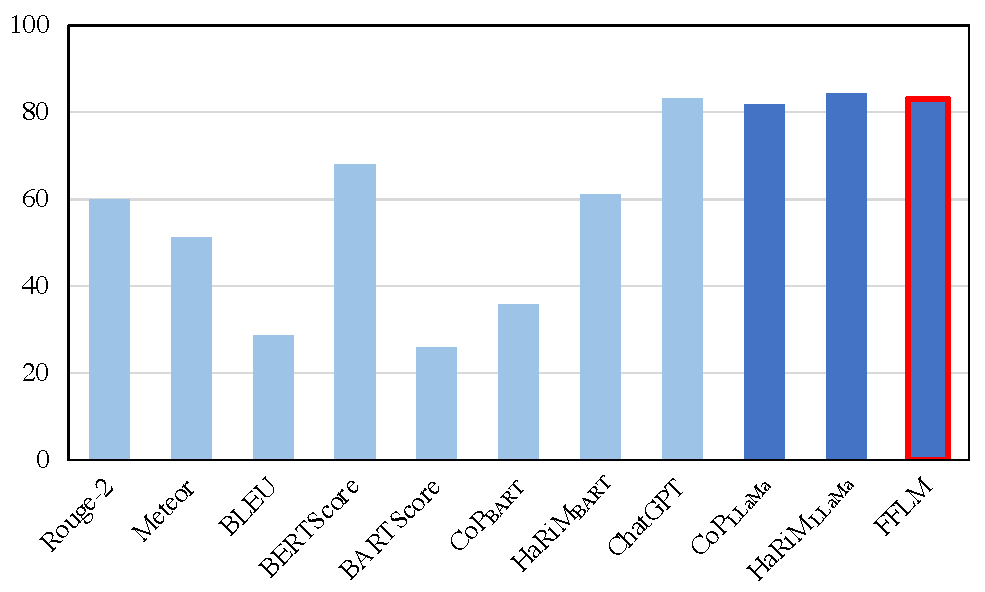
\includegraphics[scale=0.45]{system-level.pdf}
%			%\caption{fig2}
%		}%
%	\end{minipage}%
%	\caption{System-level Spearman correlation(\%) on the SummEval dataset. Dark blue represents the performance of metrics based on the foundation language model. We highlight our approach with a red box. }
%	\label{fig:systemcorrelation}
%\end{figure}



\begin{table*}[th]
	\scriptsize
	\centering
	\begin{tabular}{l|ccc|ccc|ccc|ccc|ccc}
		\toprule[1pt]
		& \multicolumn{3}{c}{FRANKCNN} & \multicolumn{3}{c}{QAGSCNN}  &  \multicolumn{3}{c}{SummEval}  & \multicolumn{3}{c}{FRANKXSUM}  & \multicolumn{3}{c}{QAGSXSUM} \\
		Metric & $\gamma$ &$\rho$ & $\tau$ & $\gamma$ &$\rho$ & $\tau$ & $\gamma$ &$\rho$ & $\tau$ & $\gamma$ &$\rho$ & $\tau$ & $\gamma$ &$\rho$ & $\tau$ \\
		\hline
		FFLM &  \textbf{62.2} & \textbf{56.0} & \textbf{43.7} & 72.3 & 65.3 & 53.0 & \textbf{56.3} & \textbf{46.9} & \textbf{37.4} & 27.0 & 25.3 & 20.6 & 28.3 & 27.1 & 22.2 \\
		
		\hline
		\multicolumn{16}{l}{\textit{Ablations on the metric components}} \\
		$\Delta_Y^{prior}$ & 32.0 & 26.4 & 20.1 & 11.9 & 7.5 & 5.7 & 24.9 & 20.5 & 16.1 & 20.0 & 19.2 & 15.6 & 20.9 & 21.3 & 17.4 \\
		$\Delta_X^{prior}$ & 34.4 & 36.0 & 27.4 & 27.7 & 28.1 & 21.8 & 23.7 & 26.3 & 20.7 & 10.2 & 11.2 & 9.2 & 4.8 & 3.2 & 2.6 \\
		$\Delta_Y^{cond}$ & 59.9 & 54.6 & 42.7 & \textbf{74.3} & \textbf{67.9} & \textbf{55.2} & 54.8 & 46.3 & 36.9 & 24.7 & 23.3 & 19.0 & 19.4 & 18.0 & 14.7\\
		$\Delta_Y^{prior}$, $\Delta_X^{prior}$& 34.7 & 29.2 & 22.3 & 17.7 & 13.0 & 9.9 & {28.3} & {23.6} & {18.6} & 20.4 & 19.7 & 16.0 & 20.7 & 21.3 & 17.4 \\ 
		$\Delta_Y^{prior}$, $\Delta_Y^{cond}$ & 61.0 & 54.2 & 42.3 &  68.1 & 60.2 & 48.4 & 54.4 & 45.1 & 36.0 & \textbf{28.3} & \textbf{26.5} & \textbf{21.6} & \textbf{29.4 }& \textbf{28.6} & \textbf{23.4}\\
		$\Delta_X^{prior}$, $\Delta_Y^{cond}$ & 60.3 & 54.7 & 42.6 & 73.9 & 66.5 & 54.0 & 54.7 & 46.6 & 37.1 & 24.7 & 23.2 & 18.9 & 19.8 & 18.3 & 14.9 \\
		
		
		\hline
		\multicolumn{16}{l}{\textit{Ablations on the metric designs} }\\
		- w/o $w$ & 61.2 &  54.8 & 42.7 & 68.4 & 60.1 & 48.6 & 54.3 & 45.4 & 36.3 & 26.9 & 25.0 & 20.4 & 26.4 & 26.00 & 21.3 \\
		- w/o $\log$ & 57.5 & 52.3 & 40.5 & 69.2 & 60.3 & 48.5 & 56.9 & 45.9 & 36.7 & 19.7 & 17.5 & 14.3 & 11.5 & 12.2 & 10.0\\
		- w/o $w$ and $\log$ & 56.3 & 51.3 & 39.6 & 66.5 & 57.6 & 46.4 & 54.4 & 45.0 & 36.0 & 18.8 & 16.6 & 13.5 & 11.0 & 12.4 & 10.2 \\
		
		
		\hline
		\multicolumn{16}{l}{\textit{Ablations on the combination weights ($\alpha$, $\beta$, $\delta$)}} \\
		same & 60.9 & 54.0 & 42.1 & 67.5 & 58.6 & 47.1 & 54.1 & 44.9 & 35.8 & 28.3 & 26.4 & 21.5 & 29.2 & 28.7 & 23.5 \\
		
		\bottomrule[1pt]
	\end{tabular}
	\caption{Ablations of FFLM on faithfulness rating. The highest scores are in bold.} % add the similar table for Summac in appendix benchmark
	\label{tab:ablations-fr}
\end{table*}


\begin{table}[t]
	\scriptsize
	\centering
	\begin{tabular}{l|ccc} % the baselines can be changed or deleted
		\toprule[1pt]
		%Model & \multicolumn{3}{c}{Correlations} \\ % three correlations
		Metric & $\gamma$ &$\rho$ & $\tau$  \\
		\hline
		Rouge-2& 50.0 & 59.9 & 68.8\\
		Meteor& 46.7 & 51.3 & 62.1\\
		BLEU& 45.0 & 28.7 & 62.1 \\
		BERTScore& 68.3 & 68.0 & 86.8 \\
		%FactCC & \\
		%FEQA & \\
		%QAGS & \\
		%QuestEval & \\
		%DAE & \\
		BARTScore & 30.1 & 25.9 & 18.3 \\
		CoP$_{\rm BART}$& 19.9 & 35.9 & 25.0 \\
		HaRiM$_{\rm BART}$  & 75.9 & 61.2 & 45.0 \\
		ChatGPT & - & 83.3 & -\\
		\hline
		CoP$_{\rm LLaMa}$ & 88.3 & 81.8 & 63.3 \\
		HaRiM$_{\rm LLaMa}$ & 89.9 & \textbf{84.4} & \textbf{66.7}\\
		FFLM & \textbf{90.4} & 83.2 & 65.0 \\
		\bottomrule[1pt]
	\end{tabular}
	\caption{System-level correlations between metrics and human ratings on the SummEval dataset.}
	\label{tab:system-correlation}
\end{table}


We also report the system-level results on SummEval in Table~\ref{tab:system-correlation}. FFLM performs similarly to ChatGPT according to the Spearman correlation. 
HaRiM$_{\rm LLaMa}$ achieves a bit higher Spearman and Kendall correlation than FFLM, while FFLM performs better on Pearson correlation showing better linear correlation with human scores.
Moreover, FFLM is more robust than HaRiM$_{\rm LLaMa}$ on different evaluation settings considering the poor summary-level performance of HaRiM$_{\rm LLaMa}$ especially for FRANKXSUM and QAGSXSUM in Table~\ref{tab:correlation}. Another observation is that although CoP and HaRiM backed on BART perform closely with them backed on LLaMa on the summary-level evaluation, they perform poorly on the system-level evaluation. This can be attributed to the fact that metrics based on CNN/DM fine-tuned BART have inductive bias~\cite{son2022harim}. They tend to prefer summaries generated by abstractive models, while extractive models are generally more faithful. Meanwhile, metrics based on the foundation language model don't show this bias, leading to the best results for ranking summarization systems.




To recap, our FFLM generalizes well among different task settings and different datasets, showing favorable performance over the baselines. 
It is backed on LLaMa with only 7 billion parameters and performs competitively with or even outperforms ChatGPT with 175 billion parameters, which is much more efficient for faithfulness evaluation.





\subsection{Ablation Study on Metric Designs}
\label{sec:analysis-design}

We carried out ablation studies of FFLM on faithfulness rating in Table~\ref{tab:ablations-fr}. The ablation results on inconsistency detection are in Appendix~\ref{sec:appendix}.

\textbf{Ablations on the metric components:} We test different combinations of the three probability changes. The results show that $\Delta_{Y}^{cond}$ is the most powerful component of FFLM. Its combination with $\Delta_{Y}^{prior}$ ranks first among ablations on both FRANKXSUM and QAGSXSUM. Together with $\Delta_{X}^{prior}$, our metric FFLM shows over 5\% increases in Spearman correlation on QAGSCNN, 1.8\% on FRANKCNN and SummEval,  without much loss on the other two datasets, records more robust results. Moreover, combining different probability changes induces performance gains in most cases, reflecting the necessity of designing a comprehensive metric(More in Sec~\ref{sec:errortype}).

\textbf{Ablations on the metric designs:} We use $w$ and $\log$ to annotate the token-level weights and the logarithm operation introduced in Sec~\ref{sec:approach-design}. Both operations contribute to the final FFLM, where $\log$ is more effective for datasets sourced from XSum and $w$ for the others.

\textbf{Ablations on the combination weights:} For the faithfulness rating task where we empirically set the weights $\alpha$, $\beta$ and $\delta$ as 0.25, 0.25 and 0.5, we compared it with the equaling weights, i.e., $\alpha=\beta=\delta=\frac{1}{3}$. FFLM performs relatively better.



\begin{table*}[t]
	\scriptsize
	\centering
	\begin{tabular}{l|ccc|ccc|ccc|ccc|ccc}
		\toprule[1pt]
		& \multicolumn{3}{c}{FRANKCNN} & \multicolumn{3}{c}{QAGSCNN}  &  \multicolumn{3}{c}{SummEval}  & \multicolumn{3}{c}{FRANKXSUM}  & \multicolumn{3}{c}{QAGSXSUM} \\
		Metric & $\gamma$ &$\rho$ & $\tau$ & $\gamma$ &$\rho$ & $\tau$ & $\gamma$ &$\rho$ & $\tau$ & $\gamma$ &$\rho$ & $\tau$ & $\gamma$ &$\rho$ & $\tau$ \\
		\hline
		$\Delta_Y^{prior}$, $\Delta_X^{prior}$& 44.7 & 46.2 & 32.0 & 32.5 & 35.8 & 23.8 & 29.5 & 34.4 & 23.7 & 28.3 & 31.1 & 20.9 & 28.0 & 24.9 & 17.0 \\ 
		$\Delta_Y^{prior}$, $\Delta_Y^{cond}$ & 26.5 & 19.9 & 12.9 &  14.7 & 2.3 & 1.2 & 20.1 & 15.6 & 10.1 & {23.4} & {20.1} & {13.4} & {-6.2 }& {-2.4} & {-1.5}\\
		$\Delta_X^{prior}$, $\Delta_Y^{cond}$ & 47.2 & 49.9 & 34.6 & 35.2 & 41.2 & 28.0 & 36.5 & 40.6 & 27.9 & 38.7 & 38.3 & 25.9 & -0.4 & 3.8 & 2.5 \\
		
		\bottomrule[1pt]
	\end{tabular}
	\caption{Correlations between pairs of the metric components on faithfulness rating.}
	\label{tab:analysis-pairs-fr}
\end{table*}


\subsection{Analysis on Error Types}
\label{sec:errortype}

By taking a look at the correlations between pairs of the metric components in Figure~\ref{tab:analysis-pairs-fr}, we can see that the correlations vary among different datasets. None of the pairs show a high degree of correlation, indicating that these components may capture unfaithfulness from different aspects.

To figure out if different probability changes correlate well with different error types in the generated summaries, we take advantage of labels in the FRANKCNN and FRANKXSUM datasets. \citet{pagnoni2021understanding} divides the factual errors in the generated summaries into three groups. Semantic frame errors(\textbf{Sem}) include errors on the predicate, entities, and additional information about the circumstance. Discourse errors(\textbf{Disc}) consist of coreference errors and discourse link errors. Content verifiability errors(\textbf{CVer}) are closely related to extrinsic hallucinations~\cite{ji2023survey}, containing the out-of-article error and grammatical error.
We randomly picked 50 error cases and 10 error cases for each error type from FRANKCNN and FRANKXSUM respectively, and mixed them with the rest faithful summaries. Spearman correlations averaged over 10 times are in Fig.~\ref{fig:error}.



\begin{figure}[t]
	\centering
	\begin{minipage}[t]{0.5\linewidth}
		\centering
		\subfloat[FRANKCNN]{
			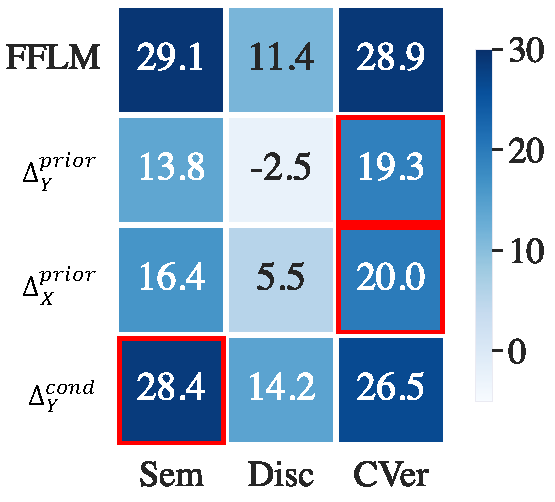
\includegraphics[scale=0.38]{error-cnn.pdf}
			%\caption{fig1}
		}%
	\end{minipage}%
	\begin{minipage}[t]{0.5\linewidth}
		\centering
		\subfloat[FRANKXSUM]{
			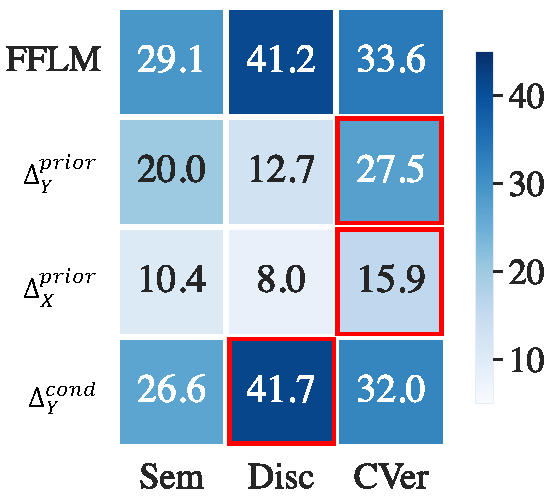
\includegraphics[scale=0.38]{error-xsum.pdf}
			%\caption{fig2}
		}%
	\end{minipage}%
	\caption{Spearman correlation(\%) of different error types on FRANKCNN and FRANKXSUM. Highest correlations for each $\Delta$ is highlighted with red boxes.}
	\label{fig:error}
\end{figure}

We observed that $\Delta_{Y}^{cond}$ captures different errors best, which is accord with the ablation results in Table~\ref{tab:ablations-fr}. Comparing among the scores for each $\Delta$ horizontally, we can see that the probability changes with prior probability is good at CVer errors on both datasets, and $\Delta_{Y}^{cond}$ at Sem errors or Disc errors. The differences among datasets reflect their different characteristics~\cite{pagnoni2021understanding}. Summaries in FRANKCNN are made up of multiple sentences, resulting in more diverse and challenging situations for Disc errors than FRANKXSUM with single-sentence summaries. Thus, $\Delta_{Y}^{cond}$  increases dramatically from 14.2\% on FRANKCNN to 41.7\% on FRANKXSUM for Disc.

FFLM made further improvements over $\Delta_{Y}^{cond}$  on both Sem and CVer, showing that combining different probability changes is reasonable and effective in most cases except Discs. 


%\begin{table}[h]
%	\scriptsize
%	\centering
%	\begin{tabular}{l|ccc|ccc}
%		\toprule[1pt]
%		 & \multicolumn{3}{c}{FRANKCNN} & \multicolumn{3}{c}{FRANKXSUM} \\
%		Metrics & Sem & Disc & CVer& Sem & Disc & CVer \\
%		\hline
%		$\Delta_1$ & 13.8 & -2.5 & 19.3 & 20.0 & 12.7 & 27.5\\
%		$\Delta_2$& 28.4 & 14.2 & 26.5 & 26.6 & 41.7 & 32.0\\
%		$\Delta_3$ & 16.4 & 5.5 & 20.0 & 10.4 & 8.0 & 15.9 \\
%		\hline
%		FFLM & 29.1 & 11.4 & 28.9 & 29.1 & 41.2 & 33.6\\
%		\bottomrule[1pt]
%	\end{tabular}
%	\caption{Spearman correlation(\%) of different error types on FRANKCNN and FRANKXSUM.} % maybe change into a figure? two 3*3 figure with different colors representing the performance
%	\label{tab:error}
%\end{table}




\subsection{Performance on Different Model Sizes}

To test FFLM's performance on different models sizes, we select LLaMa with 3 billion(3B), 7 billion(7B) and 13 billion(13B) parameters~\footnote{The corresponding checkpoints from hugging face are openlm-research/open\_llama\_3b, decapoda-research/llama-7b-hf, and decapoda-research/llama-13b-hf.} that are trained on the same data volume with 1 trillion tokens and draw the diagram in Fig.~\ref{fig:sizes-fr} for faithfulness rating datasets.
The scores consistently increase from LLaMa-3B to LLaMa-7B across the five datasets, while the improvements are not consistent for LLaMa-13B. 
Given a certain amount of data, increasing the number of parameters can enhance the model's language modeling ability and be helpful to faithfulness evaluation. On the other hand, when the model size keeps scaling up, more unexpected biases in the pre-training corpus may be memorized and will hurt the performance. 
This has also been pointed out by~\citet{ranaldi2023trip} and \citet{nadeem2021stereoset}. 

\begin{figure}[t]
	\centering
	\begin{minipage}[t]{\linewidth}
		\centering
		\subfloat{
			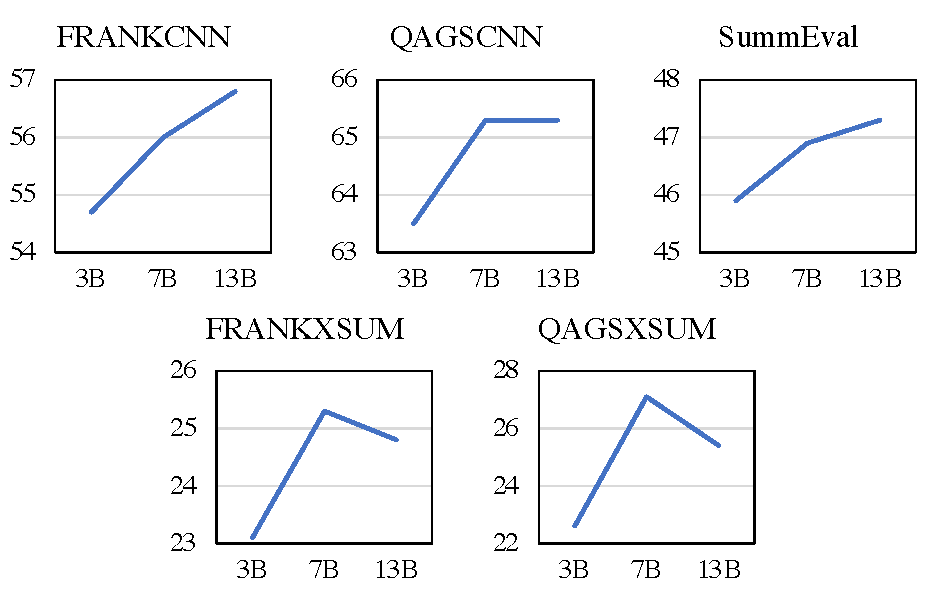
\includegraphics[scale=0.45]{sizes-fr.pdf}
			%\caption{fig2}
		}%
	\end{minipage}%
	\caption{Spearman correlation(\%) of FFLM with different model sizes on faithfulness rating datasets.}
	\label{fig:sizes-fr}
\end{figure}


\begin{table*}[t]
	\scriptsize
	\centering
	\begin{tabular}{l|ccc|ccc|ccc|ccc|ccc}
		\toprule[1pt]
		&  \multicolumn{3}{c}{FRANKCNN} & \multicolumn{3}{c}{QAGSCNN} & \multicolumn{3}{c}{SummEval} & \multicolumn{3}{c}{FRANKXSUM} & \multicolumn{3}{c}{QAGSXSUM} \\
		Metric & $\gamma$ &$\rho$ & $\tau$ & $\gamma$ &$\rho$ & $\tau$ & $\gamma$ &$\rho$ & $\tau$ & $\gamma$ &$\rho$ & $\tau$ & $\gamma$ &$\rho$ & $\tau$ \\
		\hline
		\multicolumn{5}{l}{\textit{Prompting Approach}} \\
		LLaMa-7B & -1.3 & -0.2 & -0.2 & 2.4 & 2.0 & 1.9  & 9.5 & 11.5 & 10.9 & 3.0 & 3.0 & 3.0  & -6.9 & -7.0 & -6.9 \\
		Vicuna-7B &\underline{17.6} & \underline{17.4} & \underline{15.5} & \underline{18.9} & \underline{19.8} & \underline{17.7} &\underline{13.1} & \underline{11.9} & \underline{11.1} & \underline{7.0} & \underline{5.5} & \underline{5.1} & \underline{10.2} & \underline{8.4} & \underline{8.0} \\
		Alpaca-7B &5.4 & 6.8 & 6.2 & 10.2 & 9.3 & 8.7 & 3.0 & 6.5 & 5.6 & 3.8 & 3.4 & 3.4 & 2.3 & 1.4 & 1.4 \\
		\hline
		\multicolumn{5}{l}{\textit{Our Approach}} \\
		LLaMa-7B & 62.2 & 56.0 & 43.7 & 72.3 & 65.3 & 53.0 & \underline{\textbf{56.3}} & 46.9 & 37.4 & \underline{\textbf{27.0}} & \underline{\textbf{25.3}} & \underline{\textbf{20.6}} & \underline{\textbf{28.3}} & \underline{\textbf{27.1}} & \underline{\textbf{22.2}}  \\
		Vicuna-7B & \underline{\textbf{62.7}} & \underline{\textbf{56.7}} & \underline{\textbf{44.3}} & \underline{\textbf{73.1}} & \underline{\textbf{67.2}} & \underline{\textbf{54.6}} & 55.3 & \underline{\textbf{47.2}} & \textbf{37.7} & 25.8 & 23.9 & 19.4 & 23.5 & 22.5 & 12.8\\
		Alpaca-7B & 61.4 & 55.3 & 43.2 & 71.4 & 66.0 & 52.6 & 55.8 & 47.1 & 37.6 & 26.2 & 24.6 & 20.0 & 24.2 & 25.4 & 20.7\\
		\bottomrule[1pt]
	\end{tabular}
	\caption{Comparisons with prompting and instruction-tuning techniques under the same model size. The highest correlations are in bold in each column and are underlined among each kind of approach.} 
	\label{tab:prompt}
\end{table*}


In this way, we think that using larger foundation models may not be the best choice for faithfulness evaluation on summarization, which is also closely related to the research on investigating the optimal model size and dataset size for training foundation language models~\cite{hoffmann2022empirical}. 



%\begin{table*}[h]
%	\scriptsize
%	\centering
%	\begin{tabular}{l|ccc|ccc|ccc|ccc|ccc}
%		\toprule[1pt]
%		 & \multicolumn{3}{c}{FRANKCNN} & \multicolumn{3}{c}{QAGSCNN} & \multicolumn{3}{c}{SummEval} & \multicolumn{3}{c}{FRANKXSUM} & \multicolumn{3}{c}{QAGSXSUM} \\
%		FFLM& $\gamma$ &$\rho$ & $\tau$ & $\gamma$ &$\rho$ & $\tau$ & $\gamma$ &$\rho$ & $\tau$ & $\gamma$ &$\rho$ & $\tau$ & $\gamma$ &$\rho$ & $\tau$ \\
%		\hline
%		3b &61.8 & 54.7 & 42.8 & 69.7 & 63.4 & 51.3 & 53.9 & 45.9 & 36.6 & 24.2 & 23.1 & 18.8 & 23.2 & 22.6 & 18.5 \\
%		7b & 62.2 & 56.0 & 43.7 & 72.3 & \textbf{65.3} & \textbf{53.0} & 56.3 & 46.9 & 37.4 & \textbf{27.0} & \textbf{25.3} & \textbf{20.6 }& 28.3 &\textbf{ 27.1} & \textbf{22.2}\\
%		13b & \textbf{63.8} & \textbf{56.8} & \textbf{44.5} & \textbf{72.6} & \textbf{65.3} & 52.9 & \textbf{57.3}&  \textbf{47.3} & \textbf{37.7 }& 26.9 & 24.8 & 20.2 & \textbf{33.7} & 25.4 & 20.8\\
%		\bottomrule[1pt]
%	\end{tabular}
%	\caption{Performance of FLM with different sizes of LLaMa.} % on ranking benchmar, add the similar one for summac in appendix
%	\label{tab:modelsizes}
%\end{table*}



\subsection{Comparisons with Prompting and Instruction-tuning}
\label{sec:analysis-prompts}

We compare our metric with prompting and instruction-tuning techniques under the same model size in Table~\ref{tab:prompt} for faithfulness rating. Here, LLaMa-7B is the vanilla foundation language model. Vicuna-7B~\cite{vicuna2023} and Alpaca-7B~\cite{taori2023alpaca} are initialized from LLaMa-7B and instruction-tuned with data collected in different ways. We present the maximum scores for each dataset among different prompts designed by previous works~\cite{chen2023evaluating,gao2023human,luo2023chatgpt}. The detailed prompts for each evaluation task are listed in Appendix~\ref{sec:appendix-prompt}.




First, we observe that using models containing 7 billion parameters, FFLM outperforms the prompting approach across different models and datasets.
The prompting results here lag behind the performance of ChatGPT dramatically. This leads to the conclusion that the effectiveness of prompting approaches relies highly on much larger models, while our metric FFLM can be a cheaper alternative with smaller models.
Second, instruction tuning is important for improving the prompting approach, while is not necessary for our FFLM. It enhances the models' understanding ability on instruction templates in the prompts by further tuning with relatively small datasets. However, such manually collected datasets may contain unconscious bias and hurt FFLM's performance.